\section{Многоквантовый эксперимент ЯМР}
% Многоквантовый эксперимент ЯМР\cite{Baum1985}
% 
% \begin{figure}
%   \centering
%   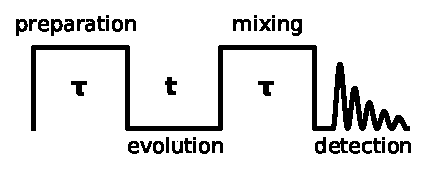
\includegraphics[width=0.5\textwidth]{mq-experiment-schema.pdf}
%   \caption{Схема МК эксперимента ЯМР}
% \end{figure}
% 
% На подготовительном периоде МК эксперимента ЯМР система облучается последовательностью радиочастотных импульсов. В результате динамика спиновой системы определяется многоквантовым гамильтонианом.
% 
% $$
% H_{MQ} = H^{(2)} + H^{(-2)},
% \quad H^{(\pm2)} = \frac 1 2 \sum_{i < j} D_{ij} I^\pm_i I^\pm_j
% $$
%     
%  МК динамику мы решили исследовать стандартным МК экспериментом.
%  Эксперимент состоит из четырех частей,
%  но нас будет интересовать только подготовительный период эксперимента.
%  На подготовительном периоде ...слайд...
% 
% Многоквантовый экперимент ЯМР
%     
% \begin{figure}
%   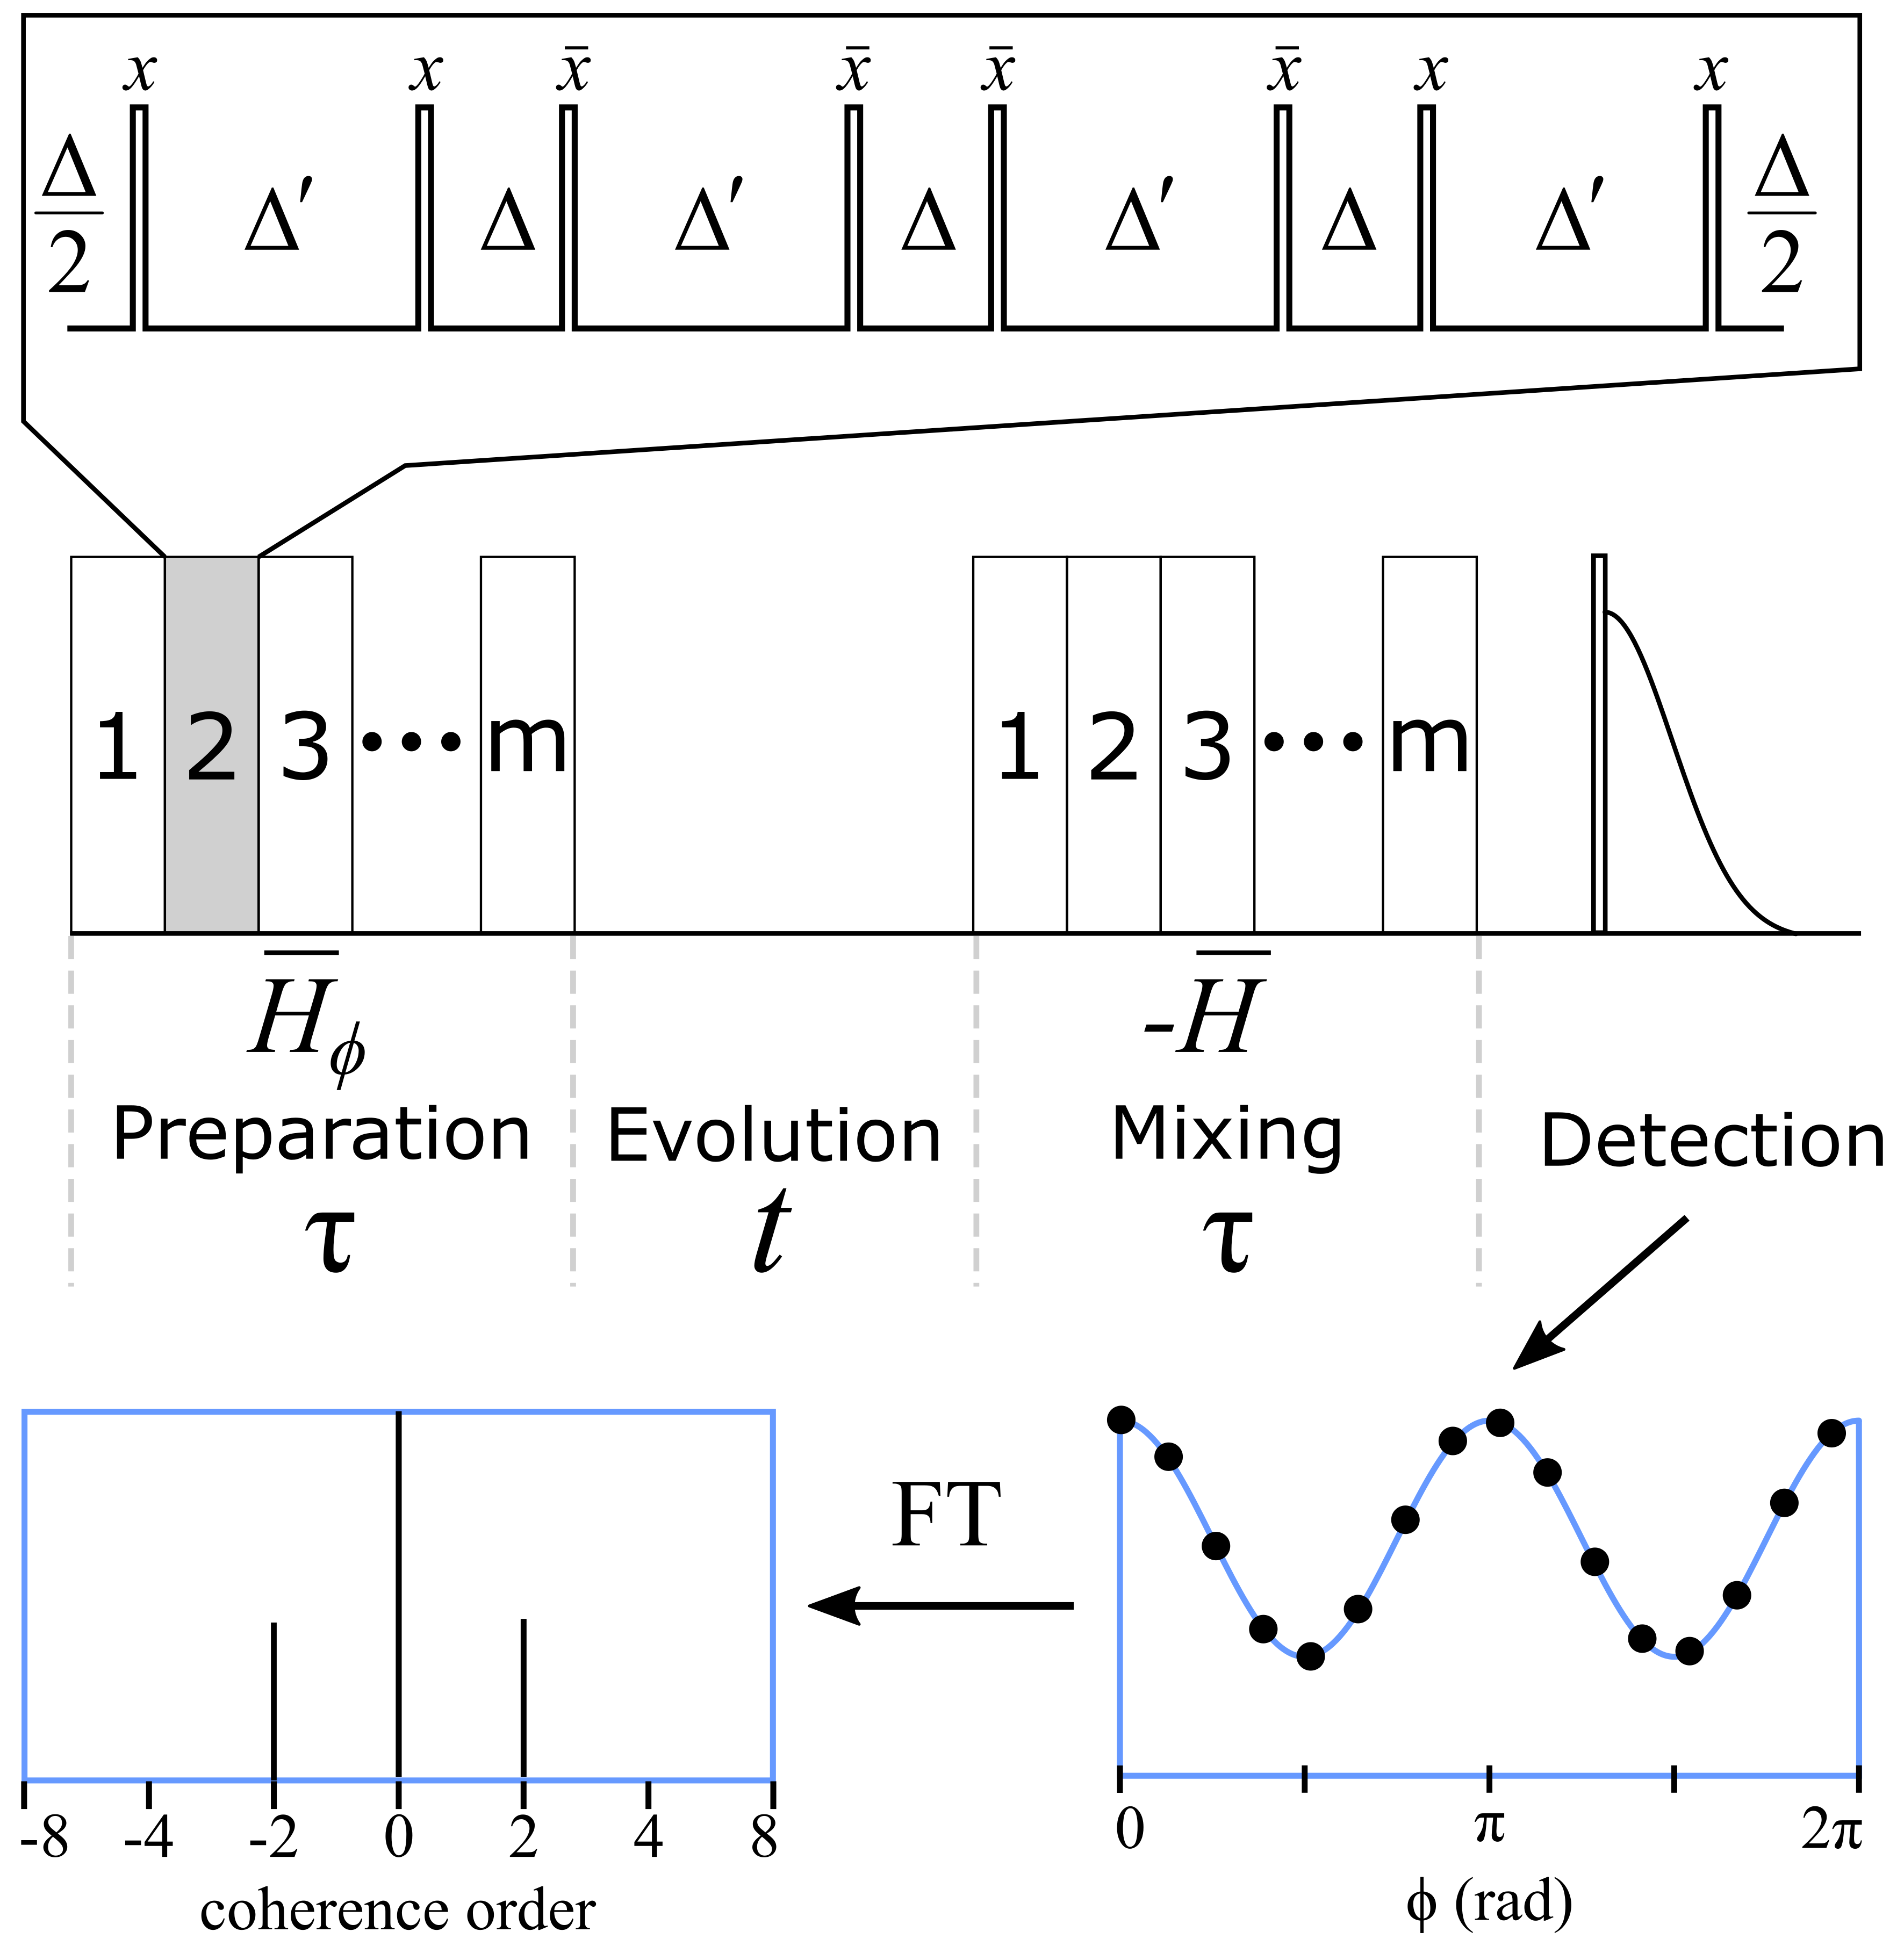
\includegraphics[width=0.9\textwidth]{mq-experiment-pulses-schema.png}
%   \caption{Схематичное представление последовательности импульсов МК эксперимента.}
% \end{figure}
%     
%     
%     МК когерентности создаются в течение периода подготовки продолжительностью $\tau$ при участии m-серии 8-импульсовых подпоследовательностей и затем преобразуются в наблюдаемую намагниченность после идентичного периода смешивания (за исключением 90-градусного фазового сдвига). Затем намагниченность детектируется при импульсе $\pi/2$. Фазовый сдвиг $\phi$ между периодами подготовки и смешивания инкриминируется для разделения многоквантовых когерентностей разных порядков. В результате преобразования Фурье по $\phi$ получается МК ЯМР спектр. Интенсивности МК когерентностей ЯМР при различных длительностях периода свободной эволюции $t$ получаются в отдельных экспериментах. 
% 
% 

\subsection{Модель эквивалентных спинов}
% Многоквантовый гамильтониан
% $$
% H_\mathrm{MQ} = - \dfrac{D}{4} \left\{
%     \left( I^{+} \right)^2 + \left( I^{-} \right)^2
% \right\}
% $$
% коммутирует с проектором квадрата полного углового момента
% $ \left[ H_\mathrm{MQ}, \hat I^2 \right] = 0 $.
% Следовательно, в базисе собственных значений  $\hat I^2$ и $I_z$  гамильтониан имеет блочно-диагональный вид :
% $$
% H_\mathrm{MQ} = \mathrm{diag} \left\{
%     H_\mathrm{MQ}^{N/2},
%     H_\mathrm{MQ}^{N/2 - 1},
%     \dots
%     H_\mathrm{MQ}^{N/2 - [N/2]}
% \right\},
% $$
% где каждый блок соответствует собственному значению полного углового момента.
% 
% Так как в нашей модели все констаны одинаковые, МК гамильтониан упрощается.
% Этот гамильтониан коммутирует ...слайд...
% 

\subsection{Дипольно упорядоченное состояние}


\subsection{Измерение информации Фишера}
% 
% % \begin{figure}
% %     \centering
% %     \includegraphics[width=\textwidth]{spin-system-energy-spectrum.png}
% %     \caption{Энергетический спектр системы}
% %     \label{fig:spectrum}
% % \end{figure}
% 
% Начальная матрица плотности в МК ЯМР. 
% %
% \begin{equation}
%     \label{eq:13}
%         \rho = \frac{1}{2}e^{\beta \omega_0 I_z} \approx
%             \frac{1}{z} \left(1 + \beta \omega_0 I_z \right)
% \end{equation}
% %
% В базисе, диагнолизирующем $\rho$, представляется в виде: 
% %
% \begin{equation}
%     \label{eq:14}
%         \rho = \sum_k \lambda_k |k\rangle \langle k|
% \end{equation}
% %
% Энергетический спектр системы дан на Рис.~\ref{fig:spectrum} 
% 
% 
% 
% В ходе эволюции системы под действием гамильтониана 
% %
% \begin{equation}
%     \label{eq:15}
%         H = H^{(2)} + H^{(-2)}
% \end{equation}
% %
% происходят переходы между энергетическими уровнями рис. 1 и возникают многоквантовые когерентности. 
% Матрица плотности $\rho_t$ $(\theta\sim t)$ при этом имеет вид 
% %
% \begin{equation}
%     \label{eq:16}
%         \rho_t = e^{-iHt}\rho e^iHt
% \end{equation}
% 
% Формулы~(\ref{eq:14}),~(\ref{eq:16}) полнотью определяют квантовую информацию Фишера согласно формуле~(\ref{eq:12}). 
% 
% % ----- 
% 
% % \begin{figure}
% %     \centering
% %     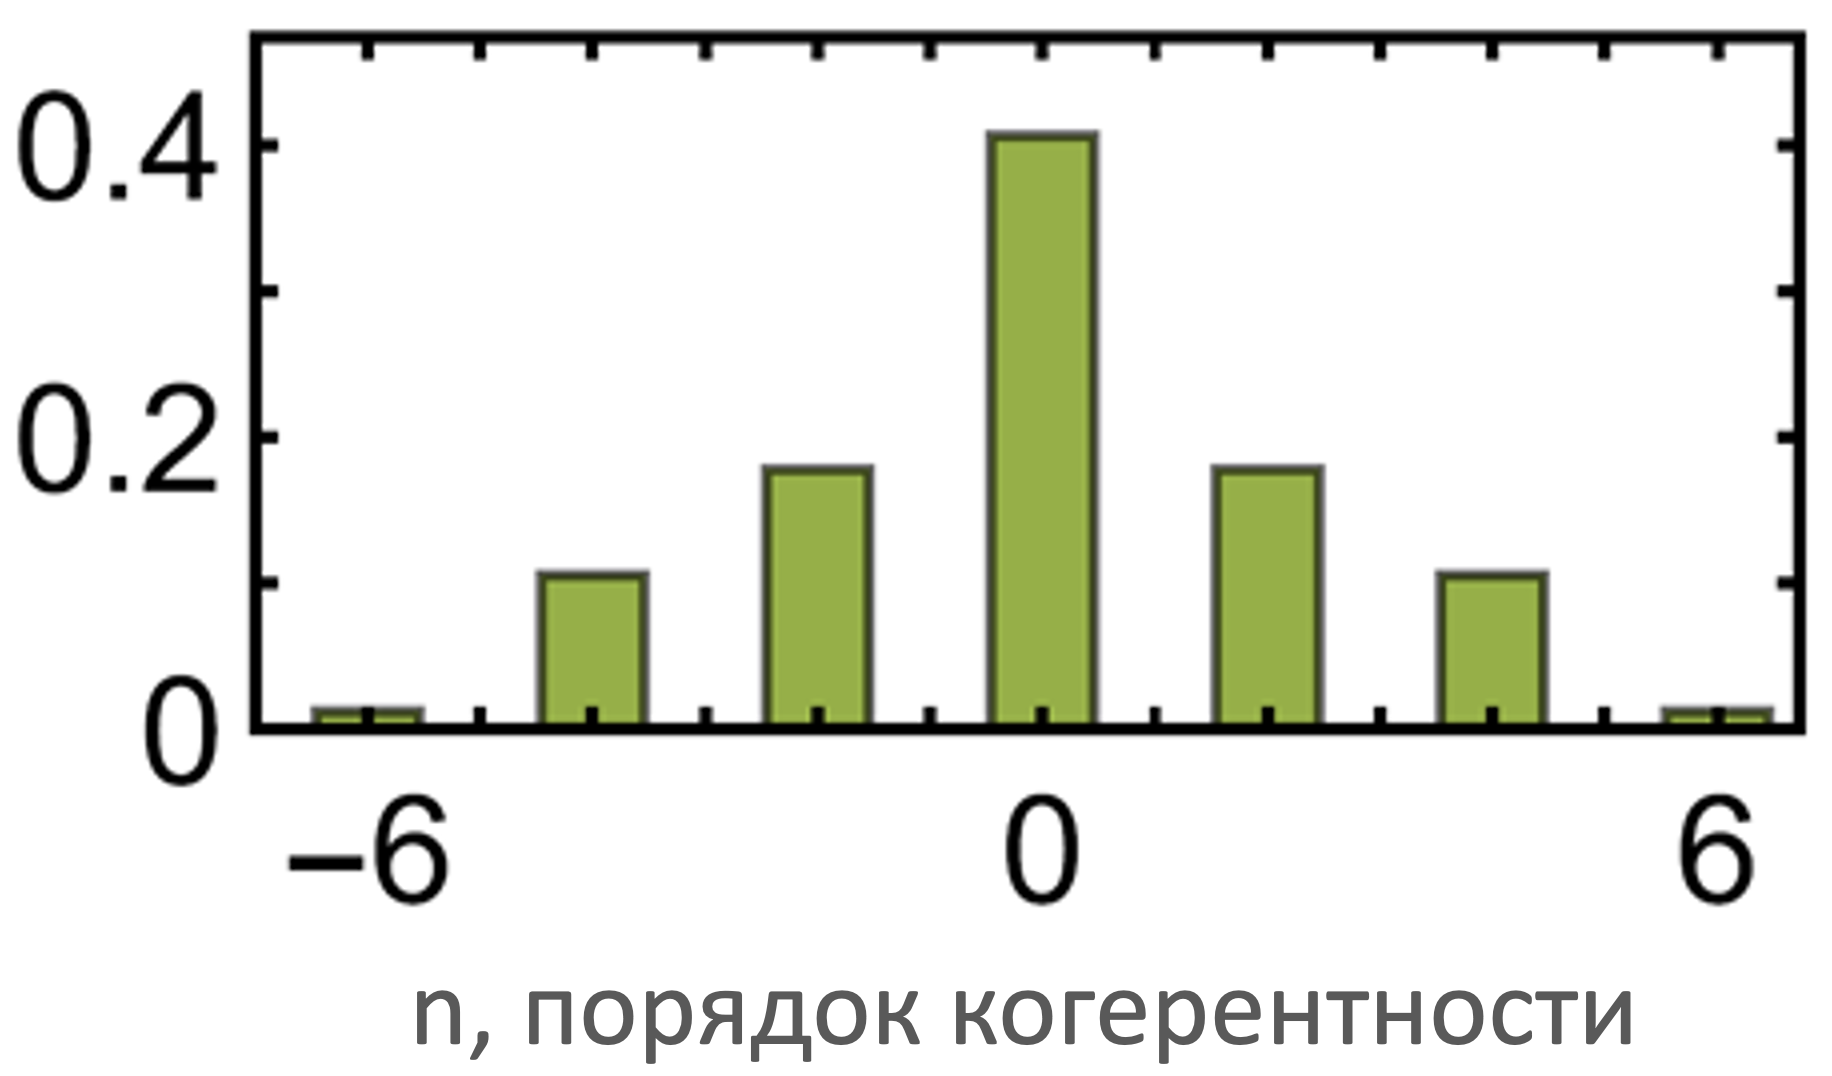
\includegraphics[width=\textwidth]{mq-coherence-intensities-hist.png}
% %     \caption{Распределение интенсивности МК когерентностей ЯМР.}
% %     \label{fig:distribution}
% % \end{figure}
% %
% \begin{multline}
%     \label{eq:27}
%         I(t) = Tr\{e^{-iHt} \rho e^{iHt} \rho\} =
%             Tr\{(1-iHt - \frac{1}{2}H^2 t^2) 
%                 \rho (1+iHt - \frac{1}{2}H^2 t^2) \rho\} \\
%                   = Tr\{ \rho^2 - it [H,\rho] + t^2 H\rho H\rho - 
%                         \frac{t^2}{2}H^2 \rho^2 - \frac{t^2}{2} \rho H^2\rho\} \\
%                    = Tr\{\rho^2\} - t^2 Tr\{\rho^2 H^2 - \rho H\rho H\} \\
%                = Tr\{\rho^2\} \left(1-t^2 \frac{Tr\{\rho^2 H^2 - \rho H \rho H}{Tr(\rho^2)}\right)
% \end{multline}
% %
% Номировка в МК ЯМР: 
% %
% \begin{equation*}
%     Tr\{\rho^2\} = Tr \left( \sum\limits_{n,m} \rho_n \rho_m \right) = 
%         Tr \sum\limits_{n} \rho_n \rho_n = 
%     \sum_n J_n (t) \equiv 1
% \end{equation*}
% %
% Второй момент~\cite{khitrin1997}: 
% %
% \begin{equation}
%     \label{eq:28}
%         M_2 = \frac{2Tr\{\rho^2 H^2 - \rho H \rho H\}}{Tr(\rho^2)} =
%             2Tr\{\rho^2 H^2 - \rho H \rho H\}
% \end{equation}
% %
% \begin{multline*}
%         2Tr\{\rho^2 H^2 - \rho H \rho H\} \\
%            = 2\sum_{j,k}\{\lambda^2_j H_{jk} H_{kj} - \lambda_j H_{jk} \lambda_k H_{kj}\} =
%                  2\sum_{j,k} (\lambda^2_j - \lambda_j \lambda_k)H_{jk}H_{kj} \\
%                    = \sum_{j,k} (\lambda^2_j - \lambda_j \lambda_k)H_{jk}H_{kj} + 
%                         \sum_{j,k} (\lambda^2_j - \lambda_j \lambda_k)H_{kj}H_{jk} \\ 
%                     = \sum_{j,k} (\lambda^2_j - 2\lambda_j \lambda_k + \lambda^2_k)H_{kj}H{jk} =
%                 \sum_{j,k} (\lambda_j - \lambda_k)^2 \left| \langle j|H|k \rangle \right|^2
% \end{multline*}
% %
% \begin{equation}
%     \label{eq:29}
%             M_2 = \sum_{j,k} (\lambda_j - \lambda_k)^2 \left| \langle j|H|k \rangle \right|^2
% \end{equation}
% %
% Вернемся к квантовой информации Фишера 
% %
% \begin{equation*}
%     F_Q = 2\sum_{j,k} \frac{(\lambda_j - \lambda_k)^2}
%     {\lambda_j + \lambda_k} |\langle j|H|k \rangle|^2
% \end{equation*} 
% %
% Поскольку $Tr(\rho) = 1$, $\lambda_j + \lambda_k \leq 1$ и 
% %
% \begin{equation}
%     \label{eq:30}
%         F_Q \geq 2\sum_{j,k} (\lambda_j - \lambda_k)^2 \left| \langle j|H|k \rangle \right|^2 = 2M_2
% \end{equation}
% 
% Таким образом, нижняя граница информации Фишера равна удвоенному второму моменту~\cite{g_arttner2018}. 
% Главным недостатком этого результата является то, 
% что связь со вторым моментом интенсивностей многоквантовых когерентностей
% работает только в высоко температурном приближении. 
% 
% 